

\documentclass[10pt,a4paper]{article}
\usepackage[utf8]{inputenc}
\usepackage[italian]{babel}
\usepackage{amsmath}
\usepackage{xcolor}
\usepackage{siunitx}
\usepackage{amsfonts}
\usepackage{amssymb}
\usepackage{graphicx}
\usepackage{siunitx}
\usepackage[left=2cm,right=2cm,top=2cm,bottom=2cm]{geometry}
\newcommand{\rem}[1]{[\emph{#1}]}
\newcommand{\exn}{\phantom{xxx}}
\renewcommand{\thesubsection}{\thesection.\alph{subsection}}  %% use 1.a numbering

\author{Gruppo 1G.BN \\ Massimo Bilancioni, Alessandro Foligno, Giuseppe Zanichelli }
\title{Es06B:Usi non lineari dell’ OpAmp }
\begin{document}
	\date{8 novembre 2018}
	\maketitle
	
	
	\section*{Scopo dell' esperienza}
	Scopo dell'esperienza è l'analisi di circuiti che fanno usi non lineari dell'Amplificatore Operazionale




\section{Ampificatori di Carica}
	\subsection{Montaggio circuito e valore delle componenti}
		Si monta il circuito sulla basetta.
		I valori delle varie componenti sono i seguenti:



$C_T=0.967\pm 0.04$ \si{\nano\farad} \\


$C_F=0.958\pm 0.04$ \si{\nano\farad}\\


$R_2=99.9\pm 0.9 $ \si{\ohm}\\$R_1=0.392 \pm0.03   $ \si{\mega \ohm}\\
				
Il potenziometro ha una resistenza massima di circa 1\si{\mega\ohm}.


		
Nel montaggio, si è preferito l'utilizzo di una resistenza $R_1$ circa 4 volte maggiore del valore consigliato, per poter rallentare il processo di scarica e prolungare la durata del segnale alto in uscita.
		Questo infatti, era parzialmente deformato dallo slew rate dell'amplificatore, riducendo la precisione delle misure di tempi riportate in Sezione \ref{Output} .
	\subsection{Segnale $V_{sh}$}
		Studiando il circuito, ci si aspetta, in $V_{discr}$ un'onda quadra di duty cycle variabile e ampiezza data dalle tensioni di alimentazioni dell'op-amp, dove il segnale alto indica quando il segnale in $V_{sh}$ è sopra la soglia.
		Per quanto riguarda la prima parte del circuito, anzitutto osserviamo che, ad ogni cambio di polarità dell'onda quadra, viene iniettata nel circuito una quantità di carica pari a $Q=V_{pp} C_T$. trattandola come un'iniezione istantanea, la  corrente che passa per la resistenza è trascurabile rispetto a quella che finisce sul condensatore perchè il tempo di scarica $R_1 C_F \gg$ durata dell' impulso.
		Dopo che il condensatore riceve la carica$Q$ inizia a scaricarsi su $R_1$. 

Ci si aspetta, quindi, come ampiezza massima del segnale $V_{sh}$, $V_{max}=\frac{Q}{C_F}=2 V_{in} \frac{C_T}{C_F}\approx 2 V_{in} $ dato che le capacità sono più o meno uguali. Infatti, con un'onda quadra in ingresso $V_{in}\approx3V$ si osserva il segnale $V_{sh}$ riportato in Figura \ref{fig:sample}, di ampiezza $\approx 6V$.
		
		\begin{figure}
			\centering
			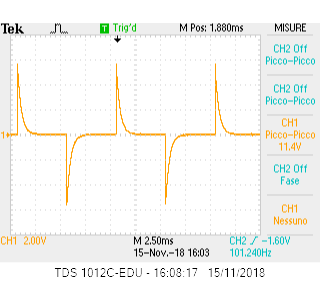
\includegraphics[scale=0.85]{sample.png}
			\caption{segnale $V_{sh}$}
			\label{fig:sample}
		\end{figure}
	\subsection{Output} \label{Output}
	
		Il segnale che si osserva come output esce da un comparatore.
		All'ingresso $V_-$ del comparatore c'è un segnale di soglia  ottenuto per mezzo di un partitore di tensione variabile. Detta $x$ la resistenza variabile del potenziometro, vale $V_{soglia}=\frac{V_E x+V_C(R_3-x)}{R_3}$ che quindi può variare fra gli estremi $V_E$  e $ V_C$.
		Il segnale sarà in alto quando vale :\[V_{soglia}\le V_{sh}=2V_{in} \frac{C_T}{C_F} \exp(-t/(R_1 C_F))\]
		\[t_{alto}=R_1 C_F \ln(\frac{2 V_{in} C_T}{V_{soglia} C_F})\] 
		Quindi si osserverà segnale alto solo se $V_{soglia} <2 V_{in} \frac{C_T}{C_F}\approx 2 V_{in} $.

In particolare, ci si aspetta anche una dipendenza logaritmica per $t_{alto}$ da $V_{in}$ e $V_{soglia}$, la prima di queste è stata verificata con le seguenti misure:
\begin{center}
\begin{tabular}{|c|c|}
	
	\hline 
	$\Delta t [ms]$ & $V_{in}[V]$ \\ 
	
	\hline 
	$1.13\pm0.01$ & $2.00\pm0.04$ \\ 
\hline 
	$1.26\pm 0.02$ & $2.76\pm0.04$ \\ 
\hline 
	$1.38\pm0.02$ & $3.80\pm0.08$ \\ 
	\hline 
	$1.56\pm0.02$ & $6.16\pm0.12$ \\ 
	\hline 
	$1.64\pm0.02$ & $7.60\pm0.16$ \\ 
	
	\hline 
	$1.72\pm0.02$ & $9.20\pm0.16$ \\ 
	\hline 

\end{tabular} 
\end{center}

\begin{figure}[h] \centering
	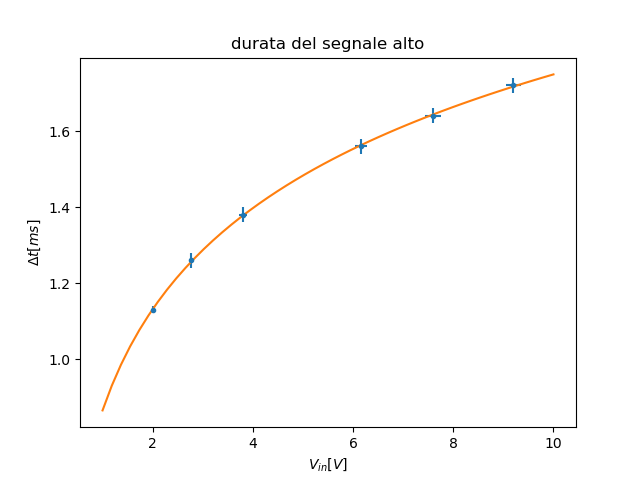
\includegraphics[scale=0.7]{Figure_1.png}
\end{figure}.\\
Come si vede, le misure hanno l'andamento predetto. \\Un fit rozzo (ci sono solo sei dati) restituisce i valori di \[R_1 C_F=(0.384\pm0.003) ms \] \[(R_1 C_F)_{expected}=(0.376\pm0.015) ms\] 
\[V_{soglia}=(104.7\pm2.5) mV\]


\subsection{Opamp non ideale}
	Si è voluto verificare che l'uscita smette di essere alta nel momento in cui i due ingressi dell'amplificatore sono allo stesso potenziale. Per far questo si è guardato sull'oscilloscopio l'intersezione fra uscita e $V_{sh}$, come riportato in Figura \ref{220mv}.
\begin{figure} \centering
	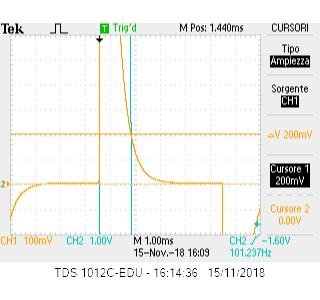
\includegraphics[scale=0.9]{220mv_2.png}
		\caption{$V_{sh}$ è in arancio, $V_{out}$ in blu}
	\label{220mv}

\end{figure}
Come si può vedere, l'uscita passa in basso per $V_{sh}\approx200mV$ (Cursore 1). Tuttavia la tensione di alimentazione misurata (sempre con l'oscilloscopio), riportava un valore superiore di circa $220mV$ e non compatibile con l'errore di misura.\\ Questo si può giustificare considerando lo slew rate dell'amplificatore, che sposta l'intersezione col segnale $V_{sh} $ più a destra, riducendone il valore.

Stimiamo l'ordine di grandezza dell'errore dovuto allo slew rate :  la linea blu è spostata a destra di qualcosa dell'ordine del $1\si{\micro\second}$ rispetto all'istante in cui i due segnali sono uguali; il tempo di scarica è $\sim 400\si{\micro\second}$ e $\Delta V \sim 6 \si{\volt} $ quindi l'errore commesso sarà dell'ordine dei $ \frac{1\si{\micro\second}}{400\si{\micro\second}} 6 \si \volt \sim 15 \si{\milli \volt}$.
\section{ Multivibratori }


\subsection{Funzionamento}
I valori misurati di $R_1$, $R_2$ e $R_3$ sono:
\[ R_1 = (9.75\pm 0.08)\si{\kilo\ohm} \qquad  R_2 = (9.98 \pm 0.08)\si{\kilo\ohm} \qquad   R_3 = ( 0.994 \pm0.001 ) \si{\kilo\ohm}\]
  Il circuito ha 2 stati possibili: condensatore che si carica e condensatore che si  scarica. L'OpAmp è configrato come un invertitore e quindi nessuno dei due stati è stabile: quando il voltaggio al capo del condensatore ha raggiunto il livello dato dal partitore di tensione $R_1/R_2$ il sistema passa nell'altro stato, con un tempo caratteristico dato dallo slew rate dell'OpAmp, dell'ordine di $10 \si{\volt\per\micro\second}$. Essendo i voltaggi usati nelle decine di volt non dovrebbe dare problemi fino a frequenze dell'ordine del centinaio di kilohertz.\label{slew_rate_count}
Il periodo di oscillazione del circuito è : \[ T = 2 RC \log( 1+ 2 R_2/R_1) \approxeq 2.23 RC\]
\subsection{Montaggio circuito}
Per ottenere un periodo di $\approx 2 \si{\milli\second}$ abbiamo scelto i seguenti valori per la resistenza e la capacità:
\[ R = ( 46.0 \pm0.5 )\si{\kilo\ohm} \qquad   C = (21.3\pm0.9 )\si{\nano \farad}\]

( $R \ll 1 \si{\mega\ohm}$ , ossia trascuriamo l'influenza dell'oscilloscopio collegato al circuito)

a cui corrisponde un periodo di oscillazione teorico:
\[T_{att}= (2.18\pm 0.14 )\si{\milli \second}\]
Inoltre abbiamo aggiunto il resistore variabile in serie a R, lasciandone un pin libero. In questo modo abbiamo potuto variare R a piacimento tra $46 \si{\kilo\ohm}$ e $146 \si{\kilo\ohm}$ per apprezzare la variazione della funzione d'onda risultante.


\subsection{Osservazioni del circuito}
Abbiamo collegato le uscite della basetta a $V_{out}, V_{+}, V_{-}$. Nel seguito potete vedere il segnale in uscita (Figura \ref{fig:V_out}) e un confronto tra $V_{+}$ e $V_{-}$ (Figura \ref{fig:V+V-}) Per questa scelta di $R$ e $C$ l'influenza dello slew rate sul periodo di oscillazione è trascurabile; non lo è invece per il seguente fenomeno: l'inversione fase carica/scarica si dovrebbe avere quando i due segnali $ V_{+}, V_{-}$ sono uguali, in realtà i valori  picco-picco differiscono per circa $\sim 100 \si{\milli \volt}$ nel senso che $ V_{-}> V_{+}$; questo succede perchè il condensatore, a causa dello slew-rate,   dopo aver raggiunto $V_+$ continua a caricarsi per un tempo molto breve prima di passare alla scarica. 

 
 \begin{figure}[h]
 	\centering
 		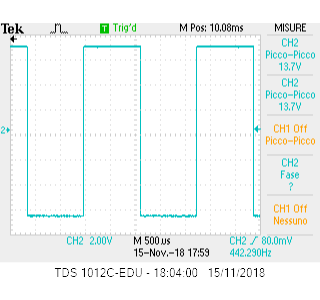
\includegraphics[scale=0.8]{vout_punto2.png}
 		\caption{\small segnale $V_{out}$ del multivibratore astabile }
 		\label{fig:V_out}
 \end{figure}
 
 \begin{figure}[h]
 	\centering
 		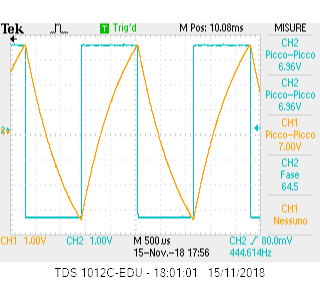
\includegraphics[scale=0.8]{v+_v-.png}
 		\caption{\small i segnali $V_+$( in azzurro ) e $ V_-$ ( in arancione )  multivibratore astabile}
 		\label{fig:V+V-}
 \end{figure}
Le misure picco picco per  segnali  $V_{out}, v_{+}$ e $v_{-}$ sono :
\[ V_{out,pp}= (13.6\pm 0.2)\si{\volt} \qquad  v_{+,pp}= (6.88 \pm 0.12)\si{\volt} \qquad   v_{-,pp}= ( 7.04 \pm0.08 ) \si{\volt}\]
Il periodo dell'oscillazione misurato sull'oscilloscopio da come risultato :
\[ T = (2.26 \pm 0.02)\si{\milli \second}\]
in accordo con il periodo teorico calcolato in precedenza.

\subsection{Motivazione degli Zener} 
La serie dei due  diodi  Zener back-to-back limita l'escursione in tensione, infatti deve essere

 $|V_{out}| \le V_{conduz} +V_{zen} = V_{Max}$. In questo modo il voltaggio in uscita ha un plateau a $V_{out} = \pm V_{max}$ generando l'onda quadra misurata.

 Dato che la resistenza dei diodi si annulla quando la tensione all'uscita dell'OpAmp supera $V_{max}$,si ha il rischio di cortocircuito. $R_3$ evita proprio questo limitando la corrente in uscita.

Dalla misura risulta \[V_{max} = ( 6.8\pm 0.1) \si \volt\]

\subsection{Periodo dell'onda quadra in uscita}

Notiamo innanzitutto che dimunuendo la tensione di alimentazione diminuiscono i problemi dovuti allo slew-rate, ma questi erano già trascurabili inizialmente visto il grande periodo di oscillazione.


Ci sono due casi da trattare:

- Se la tensione di alimentazione rimane superiore a $V_{max}$ il periodo resta invariato, infatti si calcola secondo la formula trovata nel punto 2.a che  dipende solo dai valori delle resistenze e della capacità. 

- Se invece la tensione di alimentazione scende sotto $V_{max}$ quello che succede è che uno dei due diodi Zener va in interdizione e non fa passare corrente per quel ramo . Non è  più vero che $V_{out}$ rimane costante durante  la scarica/carica del condensatore; notiamo però che essendo $R_3 \ll( R_1 +R_2)< R$,  la caduta ai capi di $R_3$ sarà i $\ll V_{Op-Amp}$ ( potenziale all'uscita dell'Op-Amp) e quindi che $V_{out}\approx V_{Op-Amp} = $ costante. In questa approssimazione possiamo riapplicare la formula del punto 2.a e di conseguenza il periodo di oscillazione rimane lo stesso con un errore non superiore al $R_3/( R_1 +R_2) = 5\% $.

\subsection{Massima frequenza}



 


Per alzare la frequenza  si  cerca di diminuire il prodotto $RC$; i limiti che si presentano sono due: 

la capacità del circuito non può essere abbassata a valori arbitrariamente piccoli perchè c'è in parallelo la capacità della basetta che quindi rappresenta il nostro valore minimo (vedere Figura 5). Inoltre per bassi valori di $C$ il dispositivo diventa tanto sensibile all'ambiente che è possibile cambiare la frequenza in modo significativo solo passando una mano sopra di esso.


Anche nel caso di $R$ avremo una resistenza della basetta che però è molto piccola; il problema che si incontra adesso, è che abbassando di molto la resistenza aumente la richiesta in corrente e quindi la potenza che deve fornire il generatore. (vedere Figura 6 )

Quello che si fa è  diminuire contemporaneamente sia $R$ che $C$; in questo modo rendiamo molto piccolo il tratto "orizzontale" di $V_{out}$ che , a causa dello slew-rate,  cessa di essere approssimabile a un'onda quadra  e diventa più simile a un'onda triangolare.

In un periodo il  segnale all'uscita dall' Op-Amp deve passare da $+15\si\volt$ a $-15\si\volt$ per quattro volte, se  assumiamo lo slew-rate di  $13 \si{\volt\per\micro\second}$ questo richiede che il periodo sia maggiore di $T_{min} = 120\si\volt / (13 \si{\volt\per\micro\second) }\approx 10^{-5}\si\second$ e quindi la frequenza di oscillazione minore di $f_{max}\approx 100 \si{\kilo \hertz}$.
\begin{figure}[h]
	\centering
	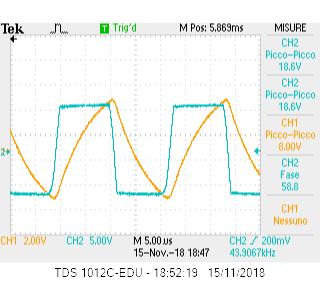
\includegraphics[scale=0.8]{basetta.png}
	\caption{\small è stato levato il condensatore lasciando solo la capacità della basetta, il valore di $R$ è quello iniziale.}
	\label{fig:basetta}
\end{figure}

Sapendo la frequenza di oscillazione si è trovato che $C_{basetta} \approx 0.2 \si{\nano \farad}$
\begin{figure}[h]

	\centering
	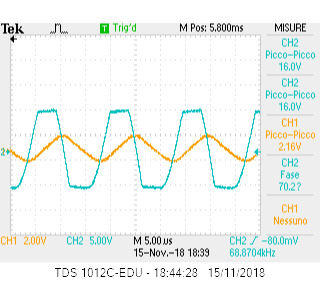
\includegraphics[scale=0.8]{freqRbassa.png}
	\caption{\small Si è abbassata la resistenza a un valore di circa $\sim 50 \si \ohm$, lasciando $C$ uguale al valore iniziale}
	\label{fig: resbassa }

\end{figure}









\end{document}  